\documentclass[usletter, 12pt]{article}
 
\usepackage{../VB}
\usepackage{cleveref}
\usepackage{caption}

%\doublespacing

\begin{document}

\lhead{\textsc{Causal Exaggeration}}

\selectlanguage{english}
	
	\title{Causal Exaggeration:\\ Unconfounded but Inflated Causal Estimates}
	
	\subtitle{Illustration of the large magnitude of exaggeration}

	\author{Vincent Bagilet}
	
	\institution{Sustainable Development PhD Program, Columbia University}

	\date{February 21, 2023}
	
	
	\maketitle
	
	
			 	 		
		\textit{To put in the introduction:}
		
		The trade-off presented in this paper only has concrete implications if the use of causal identification strategies yields substantial exaggeration, especially as compared to the amount of bias caused by confounders these methods allow to avoid. In the presence of a significance filter and when bias caused by confounders is likely to be limited and exaggeration likely to be substiantial, a biased but more precise method may lead to less bias, on average. As discussed in the introduction, \cite{ioannidis_power_2017} shows that nearly 80\% of estimates published in a wide array of empirical economic literatures are exaggerated, typically by a factor of two and one-third by a factor of four or more. On the other hand, in some settings, bias caused by confounders may not be as large. For example, \cite{weidmann_lurking_2021} documents and absence of evidence of selection bias due to unobservables in the evaluations of school programs they investigate. In such situations, if causal approaches limit too much the variation available for identification, leading exaggeration to be large, using a non causal approach may produce less bias. To further study the magnitude of exaggeration and differences between canonical causal identification strategies and other methods, I bring in a literature review I carried out in the companion paper that studies exaggeration in the case of the short term health effects of air pollution. I also develop a closer analysis of one of the papers in this literature to compare the relative magnitudes of confounding bias and exaggeration in this example.\\
		
		\textit{To put in the results section of the introduction:}
		
		I find evidence of exaggeration in this literature where larger effect sizes are found in less precise studies. The studies in this literature target different estimands, considering a wide variety of outcomes and treatments do not thus allow for a systematic review of the causal literature. I however show that only 8.4\% of the IV designs would retrieve an effect size equal to that of the corresponding naive OLS---at the conventional 80\% power threshold. This would correspond to an exaggeration factor of 4.5. The 2SLS estimators are drastically less precise than the OLS, with a median ratio of their respective standard errors of 3.8. For many studies in this literature, the causal method both reduces precision, limits statistical power and yields much larger estimates. This points towards causal exaggeration: by reducing precision, the causal identification strategies likely induce exaggeration and produce biased estimates. I then highlight the actual magnitude of the trade-off. Focusing on a particular study from this literature, I show that in this case exaggeration could be 3.1 times larger than the OVB.
						
		\section{Trade-off and Exaggeration in an Example Literature}
		
		The historical literature, composed of more than 600 studies, shows the adverse health effects of air pollution using methods mostly rely on associations \citep{dominici_best_2017, bind_causal_2019}. Newly obtained results based on causal identification strategies confirm the short-term health effects of air pollution \citep{schwartz_estimating_2015, schwartz_national_2018, deryugina_mortality_2019}. Yet, causal estimates are substantially larger than what would have been predicted by the standard epidemiology literature, with some estimates being 10 times larger. Even within a given setting, my literature review shows that the median of the ratio of the obtained Two-Stage Least-Squares (2SLS) to their corresponding ``naive'' Ordinary Least-Squares (OLS) estimates is 3.8.
		 What can explain that causal methods yield such large effects sizes as compared to non causal methods? Causal strategies could arguably remove omitted variable bias, reduce attenuation bias caused by classical measurement error in air pollution exposure or target a different causal estimand. But exaggeration could also explain part of this difference as studies on the short-term health effects of air pollution often display a low relative precision as a result of typically small effect sizes and relatively coarse data, at the city-day level \citep{peng2006model, peng2008statistical}.
		 
		 
		 \subsection{Evidence of publication bias in this literature}
		 ~
		 
		  \begin{figure}[h!]
                   	\caption{Suggestive Evidence of Publication Bias and Exaggeration in the Causal Inference Literature on Acute Health Effects of Air Pollution.}
                        \label{fig:intro}
                    	\centering
                    	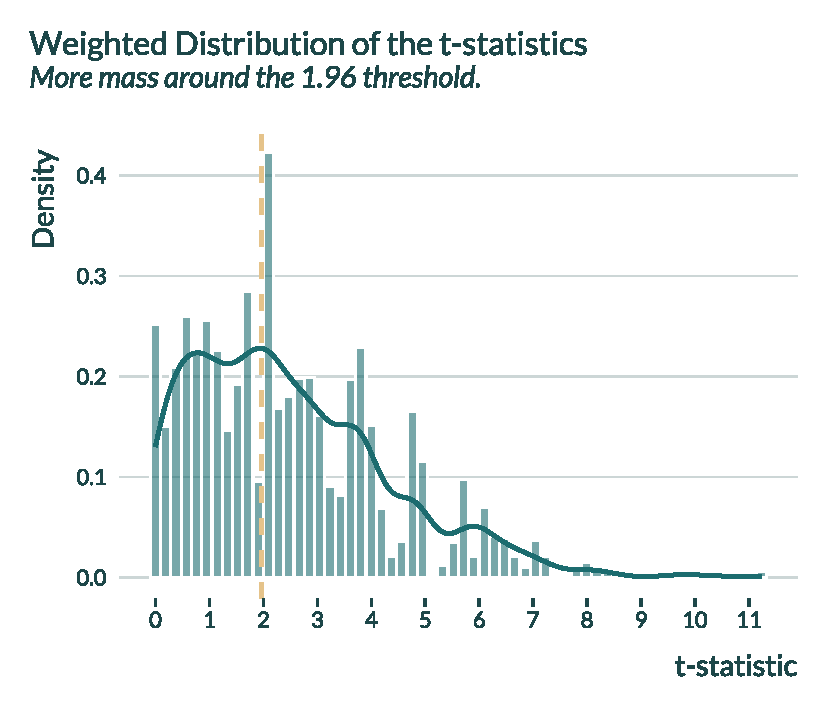
\includegraphics[width=0.48\linewidth]{images/graph_distribution_t.pdf} \ 
                    	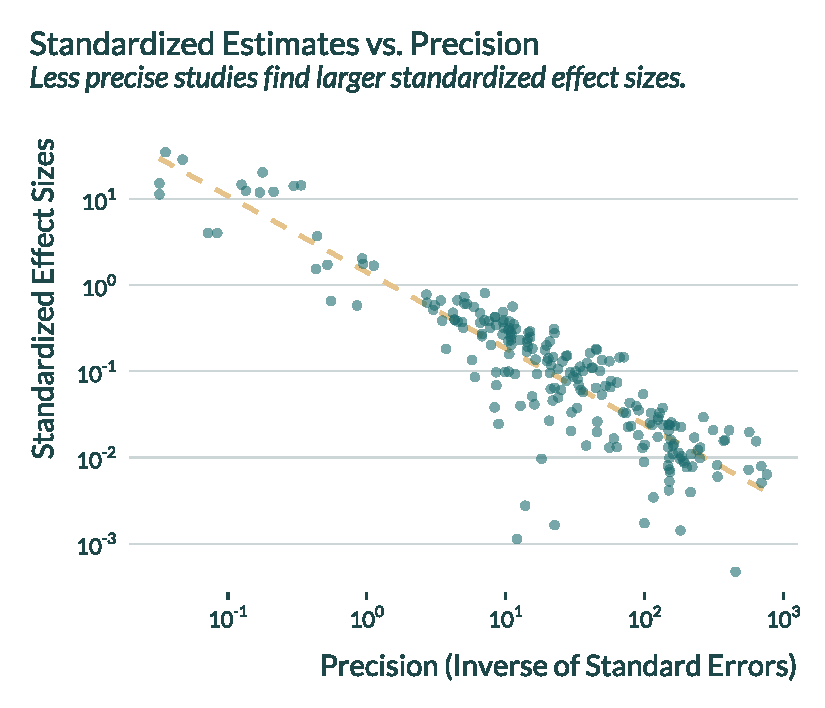
\includegraphics[width=0.48\linewidth]{images/graph_effect_precision.pdf}
                   	 \caption*{\footnotesize \textnormal{\textit{Notes}:  The sample in the left panel includes all 537 estimates reported in articles from the causal literature, including ``naive'' OLS estimates and placebo tests. Following \cite{brodeur_methods_2020}, the weights are equal to the inverse of the number of tests displayed in the same table multiplied by the inverse of the number of tables in the article. In the right panel we exclude the ``naive''  OLS estimates and placebo tests. Both axes are on a log10 scale. Limiting the sample to economics journal leaves the figures essentially unchanged (see  supplemental material). Distinguishing between top 5 and other journals shows that even if there  standardized effect sizes are typically smaller in top 5 journals, the same inverse relationship can be observed.}}
                \end{figure}
                
                The left panel of \Cref{fig:intro} reveals the presence of a publication bias in causal studies from this literature. Following \cite{brodeur_star_2016, brodeur_methods_2020} approach, I show that there is an excess mass in the \textit{t}-statistics distribution at the 5\% statistical significance threshold. The right panel of \Cref{fig:intro} produces further evidence of this favoring of significant estimates but also  points to a consequence of this publication bias: published estimates from imprecise studies might be exaggerated. In this plot we observe that less precise studies display larger standardized effect sizes. If published estimates captured true effects, their standardized effect size should be independent of the precision of the study. This figure constitutes suggestive evidence of selection on significance and exaggeration in this literature
                
                \subsection{Quantifying exaggeration}
                
                		To get a sense of exaggeration this this literature as whole, I review both the standard epidemiology and the causal inference literature but separately. I build an algorithm based on regular expressions to retrieve estimates and confidence intervals from abstracts of the former literature and perform a manual review for the second. Details on their implementation are available \href{https://vincentbagilet.github.io/inference_pollution/std_lit_getting_abstracts.html}{here}. The final corpora are composed of 2155 estimates from 668 articles and 537 estimates from 36 articles respectively.

		 	The formula for exaggeration depends on the true magnitude of the estimand of interest. To compute it, I thus need to rely on hypothesized true effect sizes. Considering the wide variety of treatments and outcomes in this literature, I cannot rely on meta-analyses to do build these assumptions. Since \cite{ioannidis_power_2017} and \cite{ferraro_featureis_2020} find a typical exaggeration of two in the economics literature, I evaluate the proportion of studies that would have a design reliable enough to retrieve an effect size equal to half of the obtained estimate. In appendix \ref{brodeur}, I implement a similar analysis on another literature, the the universe of articles published in 2015 and 2018 in the 25 top economics journals studied in \cite{brodeur_methods_2020}.
						
			If the true effect size was equal to half of the obtained estimate, 58\% of the standard epidemiology studies would have a power below the conventional 80\% target. The median exaggeration ratio would be 1.3. These figures however hide a lot of heterogeneity across studies. For one quarter of studies, the exaggeration would be larger than 1.9. This hypothesis on the true effect size, despite enabling to get an overview of the literature, can be viewed as arbitrary. For a subset of this literature, I thus make more informed guesses about potential true effect sizes, using results from a meta-analysis. \cite{shah_short_2015} gathered 94 studies on the effects of several air pollutants on mortality and emergency admission for stroke. I find that 63\% of the studies in \cite{shah_short_2015} have a statistical power below 80\% and that the median exaggeration ratio is 1.6.
			
			The causal literature displays an even lower power: if the true effect size of each study was equal to half of the obtained estimate, the median power would be 33\% and the median exaggeration ratio would be 1.7.\footnote{As for the epidemiology literature, since studies in this literature target different estimands, I cannot systematically use existing estimates or meta-estimates as estimate of the true effect. I however do so for a subset of the studies in the following section. For a systematic analysis, I rely on estimates obtained in the study considered, acknowledging limitations of this approach.} Only 11\% of studies would have a power greater than 80\%. One quarter of the studies would, on average, exaggerate the true effect sizes by a factor greater than 2. It is also worth noting that for the IV results in this literature, if the true effect was in fact equal to the naive estimate, the median power would only be 8.4\% and median exaggeration would reach 4.5. Only a small percentage of the IV designs would retrieve an effect size of the magnitude of the OLS. If the true effect is close to the OLS estimate, significant estimates from the IV design would be greatly biased. This can be explained by the fact that the IV drastically reduces precision; the median standard error of the 2SLS estimator is 3.8 times larger than the one of the corresponding OLS.
			 Importantly and as hinted by figure \ref{fig:intro}, some causal studies are more precise and unlikely to suffer from severe exaggeration issues. However, exaggeration may help explain the very large effect sizes sometimes observed in the causal inference literature. 
			 
			 %We then need to investigate whether 
			 
	\subsection{Illustration of the trade-off}
	
		I now illustrate the existence of a confounding-exaggeration trade-off in an actual setting by comparing the conventional bias of a non-causal analysis to the exaggeration of a corresponding causal one. IVs constitute approaches of choice to do so as most of them display a comparable IV estimate and OLS or conventional time series one. For an example study, \cite{he_straw_2020}, I compare the bias of the ``naive'' OLS to that of the IV by computing their distance to an estimate of the ``true effect'' they target.\footnote{I am currently carrying out the same analysis for other studies. However, variation in the treatments and outcome considered make comparisons challenging. In addition, the number of existing studies that correspond to the necessary criteria is limited (16). Computing summary statistics on such a small sample may be irrelevant, especially since the risk of exaggeration varies a lot across these studies. I thus plan to display results study by study.} %When the IV estimate differs from this ``true effect'', I explore whether exaggeration could explain this difference.
		%The ``true effect'' is the central piece of the analysis. 
		I first use the results of a meta-analysis of epidemiological studies as an estimate of this ``true effect'' \citep{shah_short_2015}. By pooling a number of studies carried out in various contexts, this meta-estimate might represent the average effect one may expect from such a study.  However, the studies in this meta-analysis do not rely on canonical causal identification strategies and may be thought of as suffering from counfounding. I thus consider the result of \cite{deryugina_mortality_2019}---a precise causal study that plausibly does not suffer from exaggeration--- as an alternative estimate of the true effect. Due to differences in settings, the estimands targeted by each air pollution study may however differ and the ``true effect'' in %a particular study 
		\cite{he_straw_2020} may deviate from these. 
		The present discussion is conditional on this true underlying effect being close to these.\\
		
		\cite{he_straw_2020} finds that a ``$10 \mu g.m^{-3}$ increase in PM2.5 increases mortality by 3.25\%'' (s.e. 1.43\%). Their corresponding OLS results suggest a 0.32\% increase (s.e. 0.23\%). 
For a similar increment in air pollution, \cite{shah_short_2015} and \cite{deryugina_mortality_2019} document a 1.1\% and 1.8\% increase in mortality respectively. The ``true effect'' based on \cite{shah_short_2015} is closer to the OLS estimate in \cite{he_straw_2020} than from their IV estimate. Provided that the three estimands are comparable, the bias of the IV is larger than that of the OLS. If the true effect was in fact closer to the one found by \cite{deryugina_mortality_2019}, both biases would be roughly equal and the bias of the IV still substantial.
		
		Exaggeration could explain this difference. Even if the IV estimator effectively removes all conventional biases, the design in \cite{he_straw_2020} would still yield exaggerated statistical significant estimates, close to the one they find. Figure \ref{graph_he} illustrates this point. The top panel displays the distribution of the IV estimator, assuming that it is unbiased and thus centered on the meta-estimate found in \cite{shah_short_2015}. The variance of this distribution corresponds to the variance of the IV estimator found in \cite{he_straw_2020}. Due to the lack of precision of this design, the statistically significant estimates are located in the tail of the distribution and therefore substantially exaggerate the true effect, by a factor 3.2 on average. The IV estimate found in \cite{he_straw_2020} could be one of these estimates. The bottom panel of figure \ref{graph_he} displays the distribution of the OLS estimator, assuming that it is centered around the obtained OLS estimate. I ignore exaggeration in this context but since the OLS is biased downward, inflating it would yield an estimate closer to the true effect. Regardless, any smaller positive estimate would be closer to the true effect than the IV estimate. 
				
		\begin{figure}[!h]
                   	\caption{Illustration of the Confounding-Exaggeration Trade-off in \cite{he_straw_2020}}
                        \label{graph_he}
                    	\centering
                    	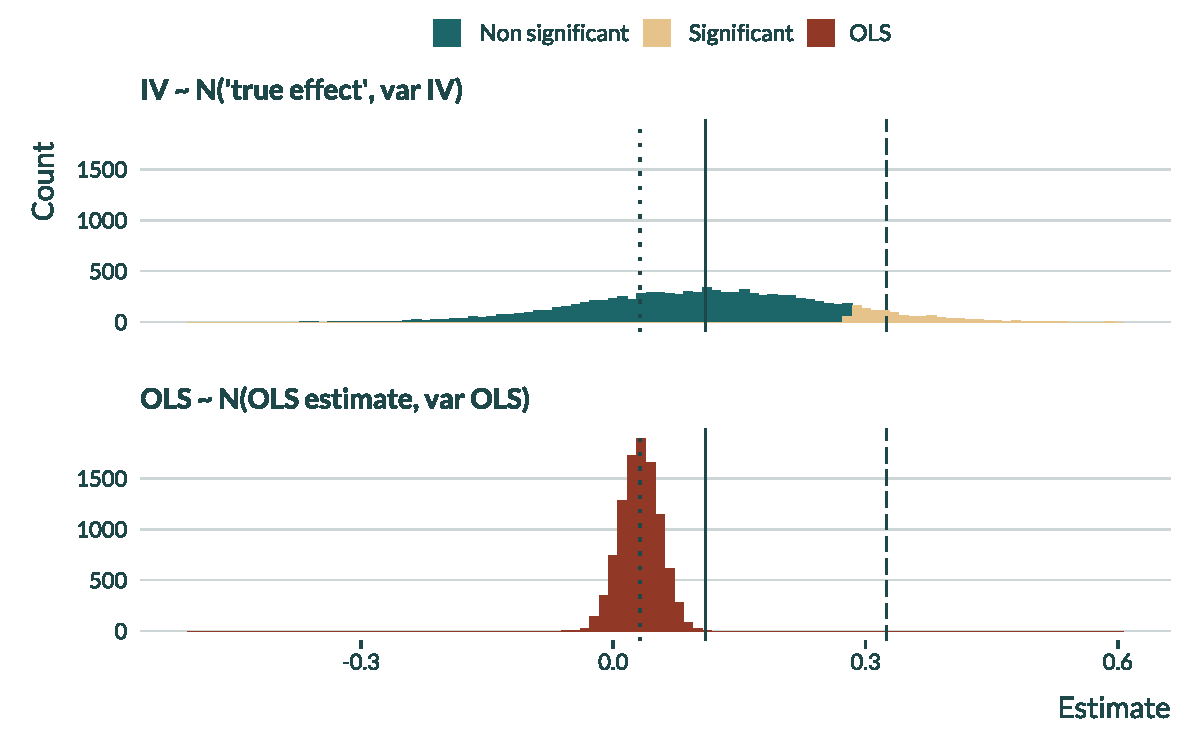
\includegraphics[width=0.8\linewidth]{images/graph_he.pdf}
                   	 \caption*{\footnotesize \textnormal{\textit{Notes}:  10000 draws from two normal distibutions. The distribution for the IV estimator is centered on the true effect, represented by the solid line and defined as the meta-estimate found in \cite{shah_short_2015}. Its variance is equal to the one of the IV estimator in \cite{he_straw_2020}. The distribution for the OLS estimator is centered on the OLS estimate found in \cite{he_straw_2020} and its variance equal to that of this same estimator. The dashed and dotted lines represent the IV and OLS estimates found in \cite{he_straw_2020} respectively.}}
                \end{figure}
				
		This example illustrates that in a published study where a causal identification strategy substantially reduces the precision of the estimator, the resulting statistically significant estimates may be further away from the true effect than the ``naive'' OLS estimate. Note that a comparable result holds if the true effect is equal to the one found in \cite{deryugina_mortality_2019}. With this design, the average exaggeration would be 3.1 times larger than the OVB (or 1.3 if the true effect is closer to the one found in \cite{deryugina_mortality_2019}).
							
			
						
			
	\newpage
	
\bibliographystyle{agsm}
\bibliography{../../causal_exaggeration.bib,pollution.bib}	

\newpage

\appendix

\section{Exaggeration by causal method}\label{brodeur}
	
	\cite{brodeur_methods_2020} analyze the universe of articles published in 2015 and 2018 in the 25 top economics journals, to evaluate differences in publication bias across methods. They find that IV and to a lesser extent DiD are particularly problematic in this regards. RDD and RCT seem to be less prone to this issue. I reinvest their data to analyze the second ingredient for exaggeration: statistical power. I carry out an analysis similar to the one carried out in the air pollution literature:  I explore whether the design of each study would enable to retrieve the true effect if it was indeed twice smaller that the one found in the study. I found that only 21\% of the studies would have the usual adequate 80\% power to select such an effect size.
	
	Decomposing across studies and under such an hypothetical effect size, I do not find substantial differences across studies, as illustrated in figure \ref{power_brodeur} and  \ref{exagg_brodeur}.
	
	  \begin{figure}[h!]
                    \caption{Distribution of hypothetical statistical power in the studies in \cite{brodeur_methods_2020}}
                        \label{power_brodeur}
                    \centering
                    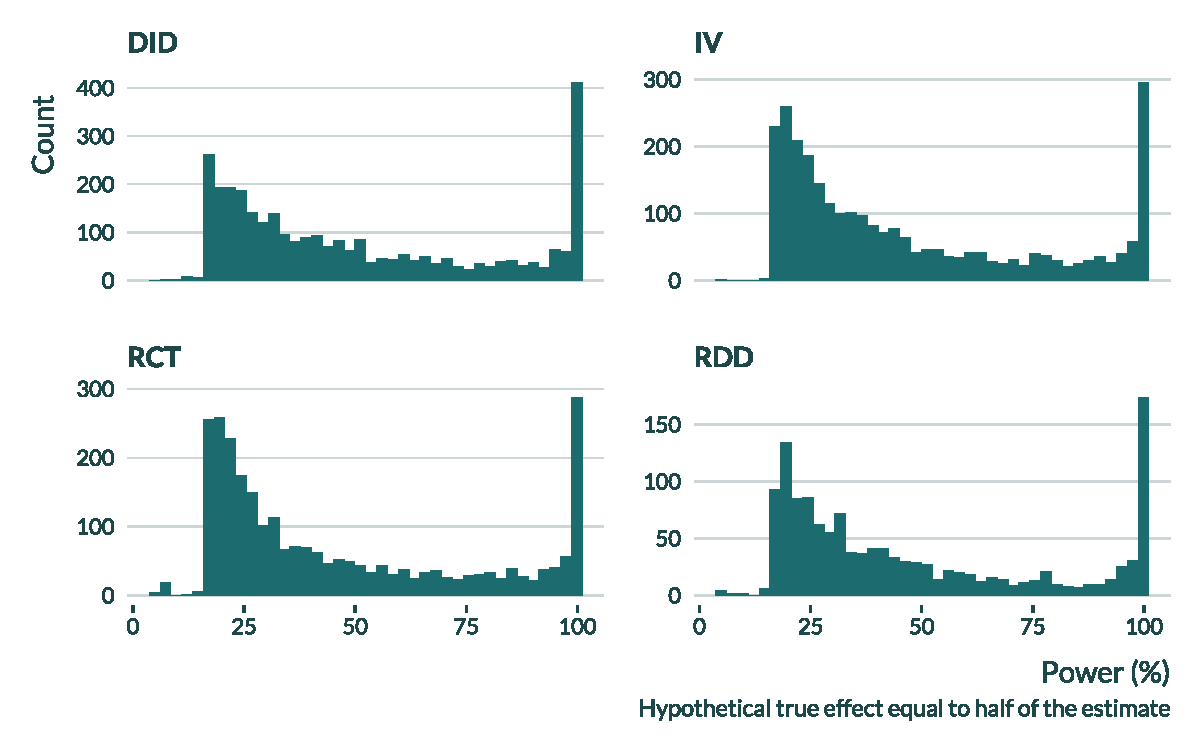
\includegraphics[width=0.8\linewidth]{images/power_brodeur.pdf}
                \end{figure}
                
                 \begin{figure}[h!]
                    \caption{Distribution of hypothetical exaggeration in the studies in \cite{brodeur_methods_2020}}
                        \label{exagg_brodeur}
                    \centering
                    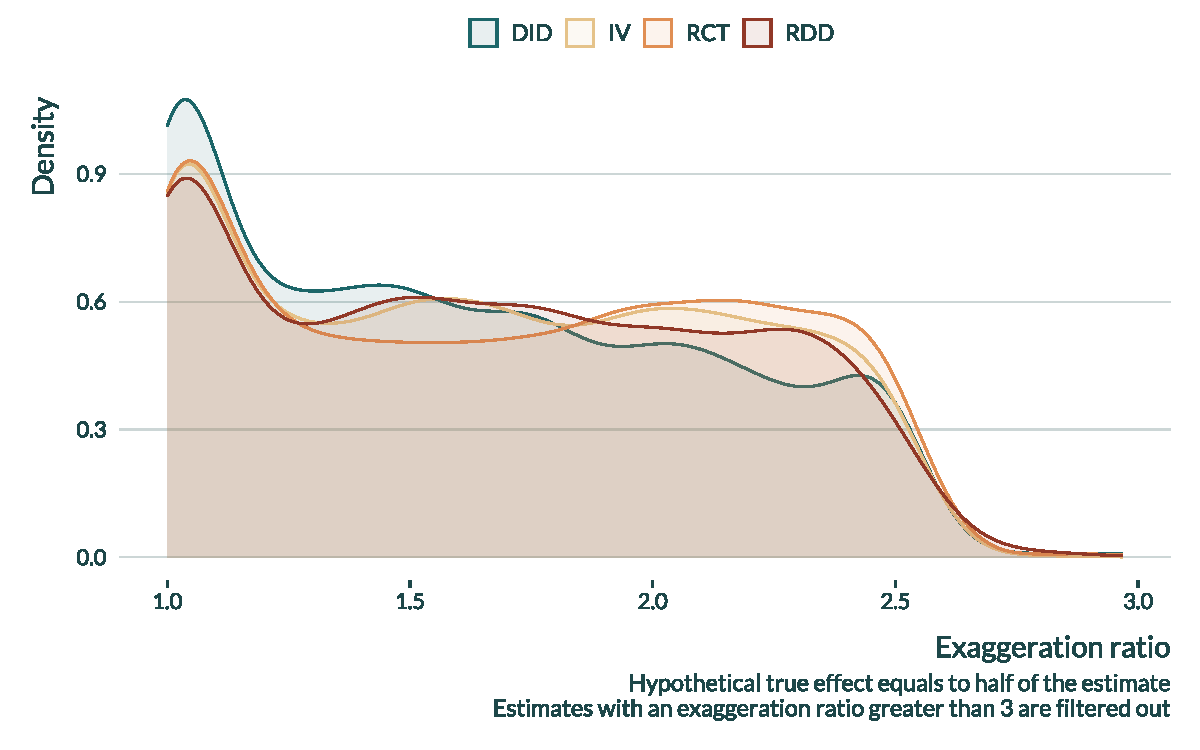
\includegraphics[width=0.8\linewidth]{images/exagg_brodeur.pdf}
                \end{figure}                
	
	
	
		
\end{document}